\documentclass[12pt]{article}

\usepackage[utf8]{inputenc}
\usepackage[francais]{babel}

\usepackage{caption}
\usepackage{subcaption}

\usepackage{tikz}

\usetikzlibrary{calc}

\usepackage[natbib=true,sorting=none,style=numeric,url=false,doi=false,isbn=false]{biblatex}
%\addbibresource{references}
\bibliography{references}

\begin{document}

\begin{titlepage}

  Stage de recherche

  {\Large \textsc{Coévolution du réseau viaire et du bâti}}

  \begin{flushright}
    \textit{Auteur :}\\
    Merwan {\scshape Achibet}\\[0.5cm]
    \textit{Encadrants :}\\
    Stefan {\scshape Balev}\\
    Antoine {\scshape Dutot}\\
    Damien {\scshape Olivier}
  \end{flushright}

  \vfill

  \begin{center}
    ILLUSTRATION
  \end{center}

  \vfill

  \begin{center}
    
\includegraphics[width=3cm]{images/logo-univ-le-havre.png}
    \qquad\qquad\qquad
    
\includegraphics[width=3cm]{images/logo-litis.png}
  \end{center}

\end{titlepage}

\begin{abstract}
abstract abstract abstract abstract abstract abstract abstract
abstract abstract abstract abstract abstract abstract abstract
abstract abstract abstract abstract abstract abstract abstract
abstract abstract abstract abstract abstract abstract abstract
abstract abstract abstract abstract abstract abstract abstract
abstract abstract abstract abstract abstract abstract abstract
abstract abstract abstract abstract abstract abstract abstract
abstract abstract abstract abstract abstract abstract abstract
abstract abstract abstract abstract abstract abstract abstract
abstract abstract abstract abstract abstract abstract abstract
abstract abstract abstract abstract abstract abstract abstract
abstract abstract abstract abstract abstract abstract abstract
\end{abstract}

\newpage

\tableofcontents

\newpage

REMERCIEMENTS

\newpage

\section{Introduction}

PROBLEMATIQUE IMPORTANTE, DE PLUS EN PLUS

SYSTEME URBAIN = SYSTEME COMPLEXE

IDEE

La première partie présente un état de l'art de la modélisation de
systèmes urbains et se concentre particulièrement sur les méthodes à
base d'automates cellulaires tout en adoptant un point de vue
historique pour justifier l'adoption de cette structure. Le modèle
conçu dans le cadre de ce stage de recherche est ensuite présenté en
seconde partie. La troisième section aborde des problématiques
pratiques rencontrées lors de l'implémentation du-dit modèle. Enfin,
des mesures diverses sont employées pour tester et valider ce travail
dans la quatrième partie.

\section{\'Etat de l'art}

\subsection{Automates cellulaires et simulation urbaine}

La modélisation de systèmes complexes est longtemps uniquement passée
par l'usage de méthodes mathématiques; typiquement, des systèmes
d'équations différentielles. Ces techniques permettent de décrire des
lois d'évolution et d'observer, ainsi que de prédire par
extrapolation, le comportement de phénomènes du réel. Dans le cas de
modèles prenant en compte un vaste jeu de paramètres, cette approche
peut néanmoins se révéler délicate à employer. Plus intrinsèquement,
même si une telle modélisation est basée sur des observations ancrées
dans la réalité, il s'agit d'une représentation conceptuelle d'un
problème et aucune mimique des mécaniques sous-jacentes ne s'opère.

Historiquement, les prémices de l'informatique moderne et d'un tout
autre paradigme de modélisation sont à attribuer aux esprits du milieu
du vingtième siècle. Alan Turing introduit en 1936 la machine éponyme
qui, bien que purement théorique, possède un module de contrôle ainsi
qu'une mémoire et peut donc exécuter une infinité d'algorithmes. Cette
démarche se démarque de l'approche mathématique et semble plus
humaine; on ne résout pas un problème en utilisant des fonctions
associant une quantité à un résultat mais on agit véritablement sur
ses données. L'idée de base de Turing était d'ailleurs d'assimiler le
fonctionnement de sa machine au travail d'une personne remplissant les
cases d'un tableau infini CITATION.

Entraîné par cette mouvance procédurale et en réaction aux réseaux de
neurones de McCulloch et Pitts, John von Neumann introduit en 1946 le
terme d'\textit{automate} CITATION pour désigner plus généralement ces
machines CAPABLE DE?. Une sous-catégorie d'automates, les automates
fini (\textit{finite state machine}), a pour particularité de changer
sa représentation interne en fonction des traitements effectués et ce,
parmi un ensemble fini d'état ; cette qualité permettant de modèliser
de façon discrète de nombreux phénomènes naturels. John von Neumann et
Stanislaw Ulam joignent leurs travaux pour concevoir l'automate
cellulaire CITATION : un système comprenant un ensemble d'automates à
états spatialement localisés (typiquement sous forme de grille) et
interconnectés en fonction de leur proximité. Les entrées de chaque
automate correspondent alors aux états des automates voisins et de
cette organisation se dégagent de fortes relations
d'interdépendance. Le jeu de la vie de Conway en est un exemple
classique. La simplicité de ses règles, mise en contraste avec la
variété des configurations engendrées, témoigne de la richesse des
automates cellulaires CITATION.

Les automates cellulaires ont depuis été extensivement étudiés et sont
appliqués à l'étude de nombreux phénomènes biologiques, physiques et
sociaux \cite{Ganguly}. La motivation d'Ulam lors de leur conception
était d'ailleurs de modéliser la croissance de cristaux. On peut aussi
citer en exemple la simulation de la dynamique de fluides
\cite{Frisch1986}, de la croissance de tumeurs \cite{Kansal2000}, de
l'évolution d'épidémies \cite{Fu2003}, de la ségrégation de population
CITATION-SCHELLING. Leur caractère spatial laisse supposer qu'ils sont
particulièrement adaptés aux applications géographiques, et dans le
cadre de notre problématique, urbaines. Ils ne fûrent paradoxalement
pas immédiatement exploités à cet effet et c'est seulement suite à un
article de Waldo Tobler, en 1975, que le rapprochement entre les
automates cellulaires et le domaine de la géographie apparaît
clairement \cite{Tobler1975}.

Une idée très exploitée dans ce domaine est d'associer un potentiel de
transition à chaque cellule et ce, vers tous les états qu'elles
peuvent prendre. Dans les modèles déterministes, la transition vers
l'état à plus haut potentiel est appliquée tandis que dans les modèles
stochastiques, un tirage aléatoire biaisé est préféré. Le potentiel
d'une cellule à passer à un nouvel état est déterminé en fonction de
paramètres propres au modèle. Peuvent être pris en compte l'élévation
du terrain, la densité de population, la proximité d'axes routiers, la
proximité de centres urbains, l'âge des parcelle, leur valeur; en
fait, toute combinaison d'attributs relatifs à un réseau urbain. Par
exemple, dans une simulation représentant les différents types
d'usage, le passage d'une cellule à l'état \textit{résidentiel}
pourrait dépendre de la proximité des commerces et des routes et de
l'éloignement des zones industrielles. Bien sûr, un nombre élevé de
paramètres à prendre en compte requiert un couplage fin et l'impact de
chaque variable peut être pondéré. Puisque les variations
individuelles de paramètres n'émergent pas de manière transparente à
la surface de la simulation, les modèles urbains basés sur des
automates cellulaires doivent être finement calibrés et leur réalisme
est un défi en soi. Pour contourner ce problème, Yeh et Li prônent
l'usage d'un réseau de neurones pour pondérer chaque paramètre à
partir de l'analyse de données cartographiques historiques
\cite{Yeh2002}.

Il est important de noter que la simplicité du formalisme enveloppant
un automate cellulaire strict s'oppose à la qualité de la simulation,
notamment dans le cadre de modèles spécifiques
\cite{Torrens2001}. Dans ce cas, une prise de liberté quant aux
formalisme originel est autorisée, voire nécessaire, pour obtenir des
résultats satisfaisants \cite{White1998}.

La première limite que le formalisme cellulaire de base impose est la
discrétisation des états que chaque cellule peut adopter. Même si
cette caractéristique fait partie intégrante des particularités qui
confèrent aux automates cellulaires leur simplicité d'usage et
d'analyse, la description de quantités pouvant arborer un éventail
infini de valeurs est alors impossible. Plus concrètement, il est aisé
de catégoriser les cellules d'un espace selon le fait, par exemple,
qu'elles contiennent des installations humaines ou non (état booléen)
\cite{Benguigui2004,Cornu} ou de façon plus sophistiquée, en fonction
de leur type d'usage (\textit{résidentiel}, \textit{commercial} et
\textit{industriel} \cite{Lechner} et plus
\cite{Dubos-Paillard203}). Représenter des quantités réelles et des
variations continues est moins aisé. Pour symboliser plus finement la
densité au c\oe ur d'un ensemble urbain, Semboloni utilise par exemple
un automate cellulaire de dimension trois dans lequel plus une pile de
cellules actives est haute et plus la zone représentée est peuplée
\cite{Semboloni2000}. Plus généralement, on peut s'autoriser à
représenter l'état d'une cellule par un vecteur contenant des valeurs
réelles; des règles de transitions adaptées et mesurées sont alors à
mettre en place.

L'homogénéité d'un automate cellulaire fait partie intégrante de sa
définition originelle : en mettant de côté l'état qu'elles adoptent,
toutes les cellules sont identiques en forme et en structure de
voisinage. Dans le cadre de notre problématique, cette approche est
limitante car, dans une ville, les parcelles ne sont que rarement
identiques et alignées. Similairement, la notion de voisinage est
clairement à redéfinir. Pour des problèmes classiques, les voisinages
de von Neumann et de Moore sont régulièrement utilisés mais la
relation par contiguité qu'ils décrivent ne convient pas à la
représentation des liens de dépendance à plus grande échelle se
développant dans un système urbain. Le positionnement d'un bâtiment
résidentiel dans une ville se base évidemment sur le voisinage direct
des zones envisagées (on veut ajouter une maison dans un quartier
résidentiel) mais il faut aussi prendre en compte les alentours plus
distants (la centrale thermique se trouvant à 500 mètres du site peut
poser problème). Une solution possible est d'étendre les voisinages de
von Neumann et de Moore tout en conservant leur forme caractéristique
CITATION. O'Sullivan a choisi de relaxer cette contrainte de
partionnement spatial régulier pour faire un pas dans la direction du
réalisme \cite{O'Sullivan2000,0'Sullivan2001} : conventionnellement,
une cellule d'automate correspond à un sous-espace urbain ou bien une
parcelle cadastrale mais dans chacun de ces cas le modèle se base
évidemment sur une simplification grossière de l'espace étudié. Il
décide donc de donner à chaque cellule les mêmes qualités topologiques
que les parcelles qu'elles représentent, même formes, même dimensions,
même coordonnées (mais peut-on encore parler de cellules ?). Une
variété de relations de voisinage sont alors envisageables, par
voisinage au sens propre, par distance dans un rayon d'influence, par
visibilité. L'éloignement du formalisme cellulaire est drastique car
la structure perd de son homogénéité (chaque cellule est différente),
la couverture de l'espace n'est plus complète (des vides entre les
cellules apparaissent) et le voisinage diffère lui aussi. Mais
TOPOLOGIE REELLE.

IMAGE DE LA THESE O'SULLIVAN

\begin{figure}
  \begin{subfigure}[b]{.5\linewidth}
    \centering
    \begin{tikzpicture}
  \draw[step=1,gray] (0,0) grid (3,3);

  \node at (0.5,0.5) {G};
  \node at (1.5,0.5) {H};
  \node at (2.5,0.5) {I};
  \node at (0.5,1.5) {D};
  \node at (1.5,1.5) {E};
  \node at (2.5,1.5) {F};
  \node at (0.5,2.5) {A};
  \node at (1.5,2.5) {B};
  \node at (2.5,2.5) {C};
\end{tikzpicture}

    \caption{Automate cellulaire classique}
  \end{subfigure}
  \begin{subfigure}[b]{.5\linewidth}
    \centering
    \begin{tikzpicture}
  \draw (0.5,0.5) node[circle,draw] (g) {G};
  \draw (1.5,0.5) node[circle,draw] (h) {H};
  \draw (2.5,0.5) node[circle,draw] (i) {I};
  \draw (0.5,1.5) node[circle,draw] (d) {D};
  \draw (1.5,1.5) node[circle,draw] (e) {E};
  \draw (2.5,1.5) node[circle,draw] (f) {F};
  \draw (0.5,2.5) node[circle,draw] (a) {A};
  \draw (1.5,2.5) node[circle,draw] (b) {B};
  \draw (2.5,2.5) node[circle,draw] (c) {C};

  \draw (a) -- (b);
  \draw (a) -- (e);
  \draw (a) -- (d);
  \draw (b) -- (c);
  \draw (b) -- (f);
  \draw (b) -- (e);
  \draw (b) -- (d);
  \draw (b) -- (f);
  \draw (c) -- (f);
  \draw (d) -- (e);
  \draw (d) -- (h);
  \draw (d) -- (g);
  \draw (e) -- (c);
  \draw (e) -- (f);
  \draw (e) -- (i);
  \draw (e) -- (h);
  \draw (e) -- (g);
  \draw (f) -- (i);
  \draw (f) -- (h);
  \draw (g) -- (h);
  \draw (h) -- (i);
\end{tikzpicture}

    \caption{Automate cellulaire graphe}
  \end{subfigure}
\end{figure}

Une prise de liberté quant à l'aspect temporel est aussi
envisageable. Un automate cellulaire strict est synchrone, i.e. les
changements d'état de toutes les cellules s'effectuent
simultanément. Si le choix était fait de mettre à jour chaque état de
façon asynchrone, le comportement de l'automate en serait lourdement
modifié. Par exemple, les qualités auto-réplicatives de certaines
entités du jeu de la vie ne seraient pas garanties. Il est pourtant
légitime de se questionner sur la validité d'un tel choix dans une
simulation urbaine, premièrement parce qu'une ville est un système
complexe et désordonné, deuxièmement parce les processus qui s'y
déroulent sont réglés sur différentes échelles temporelles.

Bien que les automates cellulaires soient couramment utilisés pour
simuler le traffic routier (dans leur version 1D CITATION ou 2D
\cite{Queloz1996}), ils s'accordent peu avec la construction même d'un
réseau viaire. Dans les simulations cellulaires urbaines, le
positionnement des routes a un impact sur le développement des
cellules puisque le viaire attire le bâti mais le réseau est souvent
fourni en entrée et reste fixe. Nous sommes amener à nous interroger
sur la capacité des automates cellulaires à modéliser le développement
routier. Les relations de proximité les caractérisant sont-elles
adaptées à la construction de structures dont l'échelle est celle de
la ville et non plus celle de la parcelle ? Est-il bénéfique de
représenter une route par un ensemble de cellules ou plutôt par une
entité unique ? PRECISER

\subsection{Approches alternatives}

Les automates cellulaires ne sont pas l'unique moyen de modéliser la
croissance urbaine. Plusieurs simulations existantes sont des systèmes
multi-agent \cite{Lechnera,Lechner2004}. Dans ces cas, un agent est
assimilé à un promoteur immobilier et peut acheter des terres, les
vendre, les développer ou changer leur type. Les actions qu'il
entreprend sont évaluées en fonction de l'impact sur la ville
(changement de la valeur immobilière, avis de la population) et des
réglementations locales afin d'éviter toute configuration illégale.
Pour la construction du réseau routier, une solution est de mettre en
place, en plus des agents promoteurs, deux types d'agents
traceurs. Les \textit{extenders} parcourent toute la surface du
terrain à la recherche de bâtiments isolés puis tracent une route
jusqu'au réseau urbain. Les \textit{connectors} se déplacent
uniquement sur le réseau viaire et y raccordent les bâtiments non
connectés se trouvant dans leur rayon de détection
\cite{Lechnera}. PLUS?

D'autres solutions s'éloignant des systèmes complexes et penchant du
côté de la génération procédurale de contenu existent. Souvent, le
domaine d'application de telles méthodes est l'infographie, le cinéma
et le jeu vidéo et l'objectif est alors de construire de manière
automatique une ville visuellement réaliste sans se soucier de son
caractère fonctionnel. Usuellement, l'organisation parcellaire dépend
entièrement du réseau routier car la première étape est souvent de
générer un réseau viaire complet puis de placer le bâti en subdivisant
récursivement les niches vides formées par les voies. Dans Citygen
\cite{Kelly2007}, un point $p$ de l'espace est aléatoirement choisi
puis on calcule un ensemble de plusieurs routes raccordant $p$ au
réseau routier existant en faisant varier leur déviation angulaire et
un paramètre de bruit; la route finale est celle pour laquelle la
variation d'altitude est la plus faible. ECHANTILLONAGE CityEngine
\cite{Parish2001} utilise un L-System dont les règles permettent de
reproduire les différents motifs quadrillés, radiaux et organiques que
l'on retrouve dans une ville. La nature récursive des L-Systems permet
à ces motifs de se combiner et d'apparaître à différents niveaux de
profondeur; les résultats sont saisissants. Dans une autre simulation,
le tracé des routes suit les \textit{hyperstreamlines} \cite{Chen2008}
formées par un champ de vecteurs. Ce champ est calculé par combinaison
de plusieurs autres champs de vecteurs, chacun représentant des
contraintes directionnelles particulières telles que les zones
interdites (eau, espaces verts), l'altitude et la densité de
population. Ces techniques sont intrinsèquement géométriques, et comme
précisé plus haut, le résultat est purement visuel, mais elles
représentent une source d'inspiration à ne pas négliger.

Souvent, SPECIALISATION. L'un des seuls modèles gérant à la fois
l'évolution du réseau viaire et du bâti est présenté par Weber
\cite{Weber2009} et n'emploie pas d'automate cellulaire. Le principe
est le suivant : à chaque agrandissement du réseau urbain, on crée
plusieurs routes virtuelles en suivant des règles géométriques
précises (allongement des voies existantes, limitation du degré des
carrefours à 4, l'angle entre chaque rue tend vers 90 degrés). Parmi
les $n$ routes générées, une seule sera construite. Pour la choisir,
le traffic sur ces nouvelles routes est simulé par des agents piétons
et véhicules et l'on identifie celle qui sera la plus bénéfique au
réseau. AUTRES PAPIERS?

\section{Le modèle}

\subsection{Structure}

Comme énoncé précédemment, les automates cellulaires sont des
structures versatiles et puissantes dont le formalisme originel impose
néanmoins quelques limitations; l'une des principales étant, à nos
yeux, un maillage régulier et statique.

Pour répondre à notre problématique, il est nécessaire d'employer une
structure souple et dynamique permettant de représenter à la fois le
bâti et le viaire. PLUS D'ARGUMENTS. On propose à cet effet d'utiliser
le diagramme de Voronoï.

Un diagramme de Voronoï est une subdivision de l'espace basée sur
l'évaluation de distances à des points particuliers, les
générateurs. Chaque point de l'espace est considéré comme appartenant
à l'espace d'un générateur (sa cellule de Voronoï) si la distance
séparant ces deux élements est inférieure à la distance séparant le
point de tous les autres générateurs. Autrement dit, chaque point
appartient à la cellule de Voronoï du générateur qui lui est le plus
proche.

\begin{figure}[h]
  \centering
  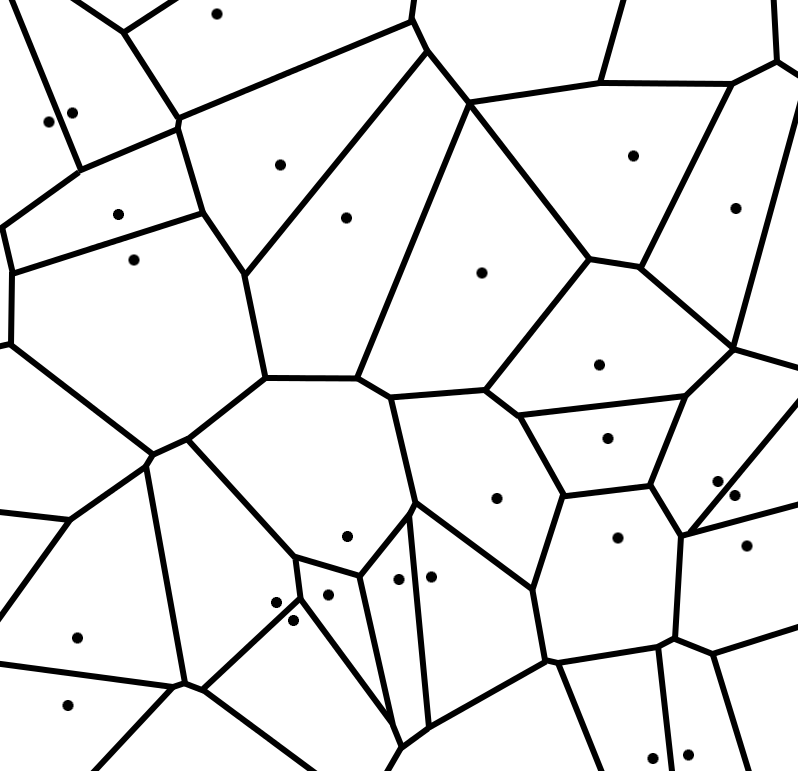
\includegraphics[width=0.5\linewidth]{images/voronoi.png}
  \caption{Un diagramme de Voronoï. Chaque cercle noir est un générateur.}
  \label{fig:voronoi}
\end{figure}

Quelques propriétés notables.

Les diagrammes de Voronoï trouvent de nombreuses applications en
science. En robotique, les obstacles présents dans un environnement
peuvent être assimilés à des générateurs et un robot cherchant à
maximiser leur évitement préférera longer les frontières des cellules
(les arêtes de Voronoï). En sociologie géographique, ils permettent
d'opposer les zones d'influence de différents éléments urbains et
répondent à des questions telles que : quel magasin un piéton
sera-t-il plus susceptible de visiter selon la zone dans laquelle il
se trouve ? En géologie, ils permettent de modéliser les écoulements
souterrains d'eau. En biologie, on les utilise pour simuler la
croissance cellulaire. DETAILS?

On remarque qu'une grille régulière, comme celles présentes dans les
automates cellulaires classiques correspond à un diagramme de Voronoï
dans laquelle les générateurs sont alignés et régulièrement
disposés. PAS TRES UTILE

Un diagramme de Voronoï représente notre espace urbain et c'est tout
naturellement que l'on imagine chaque cellule représenter une parcelle
cadastrale. L'usage du diagramme permet d'identifier les parcelles
voisines comme étant celles partageant une arête de Voronoï. Un graphe
de voisinage est ainsi construit, et adopte la forme duale du
diagramme de Voronoï : la triangulation de Delaunay. Ce premier graphe
décrit le réseau d'influences mettant en relation les parcelles
proches les unes des autres et servira à établir les relations de
voisinages régissant l'évolution de l'automate cellulaire.

Cette structure permet de décrire un canevas urbain de base mais la
composante routière est encore absente. Chaque arête de Voronoï
correspond à un espace entre deux parcelles, et est susceptible
d'accueillir une route. On choisit donc de construire un second
graphe, dual au graphe du bâti, dont les arêtes seront les routes
potentielles entre chaque bâtiment et les n\oe uds des carrefours (sur
les sommets des cellules). On l'appelle le graphe routier
\textit{potentiel}. L'évolution du réseau viaire consiste à choisir
quelles arêtes prendre dans le réseau routier \textit{potentiel} pour
les mettre dans le réseau routier \textit{construit} en fonction de
qualités internes au système.

La potentialité est une part importante de ce modèle : on choisit
quelles routes construire pour mieux servir la ville, mais aussi
quelles parcelles. À cet effet, il est nécessaire de préparer les
bords de la ville en y ajoutant des parcelles elles aussi potentielles
pour porter la morphogénèse du système. Ce placement de parcelles
invisibles se fait continuellement et permet de prévoir à court terme
l'évolution de la ville tout en laissant la sélection de quelles
parcelles construire être fonction de REFORMULER

Il est essentiel de dissocier le polygone représentant la cellule de
Voronoï associée à une parcelle et sa véritable empreinte
cadastrale. Une cellule représente l'influence d'une parcelle dans
l'espace urbain et possède comme seul point commun avec l'empreinte
son centre. Similairement, une arête indique qu'une voie passe entre
deux parcelles sans pour autant fournir ses coordonnées ou sa
courbure. Si l'on souhaite, dans un but infographique, générer une
image de notre ville à partir de ce modèle, un travail
d'interprétation est nécessaire. La figure \ref{fig:interp} illustre
ce ??? et donne, pour un diagramme de Voronoï trivial, plusieurs
interprétations envisageables. OUT OF SCOPE

\begin{figure}[h]

  \centering
  \subcaptionbox{}[0.9\linewidth][c]{
    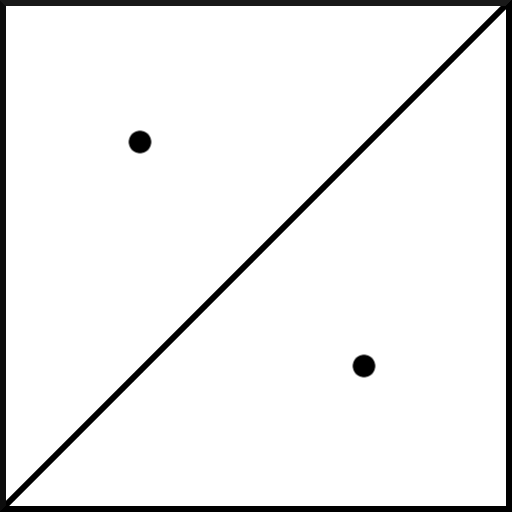
\includegraphics[width=.3\linewidth]{images/voronoi-interpA0.png}
  }

  \subcaptionbox{}[.3\linewidth][c]{
    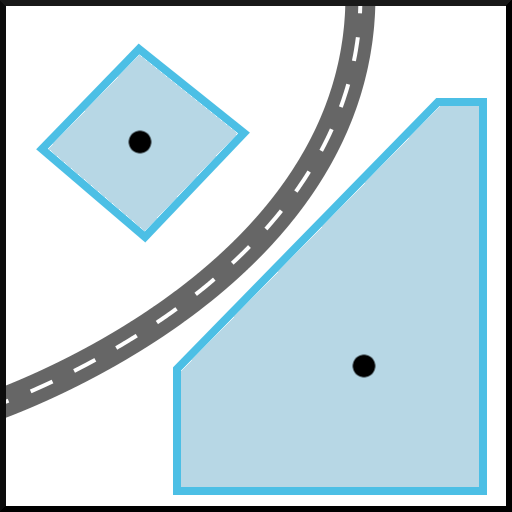
\includegraphics[width=.3\linewidth]{images/voronoi-interpA1.png}
  }
  \subcaptionbox{}[.3\linewidth][c]{
    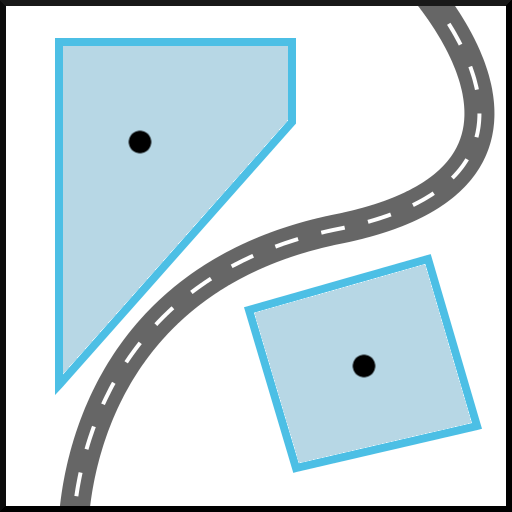
\includegraphics[width=.3\linewidth]{images/voronoi-interpA2.png}
  }
  \subcaptionbox{}[.3\linewidth][c]{
    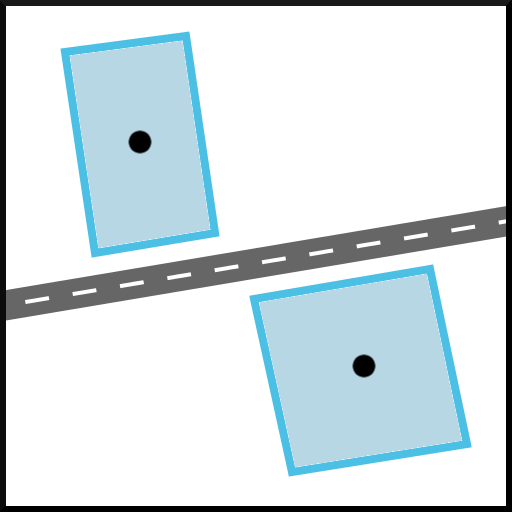
\includegraphics[width=.3\linewidth]{images/voronoi-interpA3.png}
  }

  \caption{Un diagramme de Voronoï simple et trois interprétations possibles}
  \label{fig:interp}
\end{figure}

Idéalement, ce modèle doit être capable de simuler la croissance d'une
ville déjà bien établie mais il doit aussi être possible de partir
d'une feuille blanche et de générer des villes totalement imaginaires,
notamment afin de tester les effets de différents paramètres. Autre
contrainte ; on souhaite que le modèle reste général et que toute
contrainte non prévue initialement (influence de l'altitude, de la
pente, interaction volontaire) soit aisémente prise en compte.

Ce modèle comprend quatre mécanismes distincts que l'on a voulu
généraux afin de pouvoir en altérer un sans compromettre la fiabilité
de la simulation. Trois de ces mécanismes évaluent la ville
potentielles dont l'on dispose (le réseau routier potentiel et le bâti
potentiel, donc) afin de sélectionner quels élements construire
définitivement et, au contraire, quels élements ignorer. Le quatrième
est quant à lui chargé de faire croître la partie potentielle de la
ville et donc de prévoir à court-terme l'évolution futur du système.

IMAGE !

INSISTER SUR LA POTENTIALITE

PARALLELE REEL : on prévoit des infrastructure -> on construit des
routes -> on construit les infrastructure

\subsection{Mécanismes évolutionnels}

\subsubsection{Prévision des parcelles}

\subsubsection{Expansion du réseau routier}

\subsubsection{Construction des parcelles}

\subsubsection{Automate cellulaire graphe}

\section{Construction}

Notre système urbain est décrit sur deux niveaux; plus précisément,
par deux graphes. On distingue donc le graphe parcellaire du graphe
viaire car, bien qu'ils soient étroitement liés, ils représentent des
couches différentes du réseau urbain.

\subsection{Le graphe parcellaire}

Le graphe parcellaire correspond à la couche bâti. Ses n\oe uds sont
les centres des parcelles et chacune de ses arêtes représente une
relation de voisinage entre deux parcelles.

Un diagramme de Voronoï valide est nécessaire à la construction de ce
graphe. Les seules données dont l'on a besoin en entrée sont donc les
positions centrales des parcelles. Ces coordonnées peuvent être
extraites de fichiers d'informations géographiques mais dans un
premier temps, et dans un but llustratif, on se cantonne à utiliser
des positions aléatoirement choisies.

IMAGE

La librairie Java JTS est spécialisée dans les traitements
géométriques et permet notamment de générer un diagramme de Voronoï à
partir d'une liste de points. Le résultat d'un tel traitement prend la
forme d'un ensemble de polygones, chacun représentant une cellule de
Voronoï, mais aucune autre information (d'adjacence par exemple) n'est
fournie. Une fois le graphe parcellaire peuplé par des n\oe uds
positionnés aux coordonnées fournies plus tôt, il reste donc à
calculer les relations de voisinage.

IMAGE

Puisque l'on ne dispose que des polygones formant le diagramme de
Voronoï et des positions de leur centroïdes, on procède par
l'utilisation de tests géométriques. Naturellement, si deux cellules
sont en contact -- si elle partagent une arête -- alors on relie les
deux n\oe uds du graphe leur étant associés.

IMAGE

On observe sur la figure ??? que les parcelles situées en bordure de
la ville sont dotées d'immenses cellules de Voronoï de par leur
position. Afin de ne pas influencer négativement le déroulement de la
simulation, dans laquelle l'aire des cellules peut avoir un impact sur
l'évolution du système, on préfère modifier les contours du diagramme
pour qu'il épouse la forme générale de la ville. Pour ce faire, on
calcule l'enveloppe convexe du jeu de points utilisés comme
coordonnées initiales, on l'agrandit de quelques unités afin que les
parcelles ne soient pas collées à la bordure extérieure et on conserve
uniquement l'intersection du diagramme original et de cette enveloppe.

EN FAIT, NON !

IMAGE

La finalité de cet exercice n'est pas seulement de faire évoluer
l'automate cellulaire irrégulier que forme cette structure mais aussi
de lui permettre de se transformer au cours du temps, de s'étendre par
morphogenèse. Il est donc absolument nécessaire de la dôter de
fonctionnalités d'automodification dynamiques qui modifieront les
sous-parties du graphe incrémentalement, en opposition au traitement
décrit précedemment qui ???.

UN PEU DE TRAVAIL

PAS TRES RAPIDE (MAIS PAS IMPORTANT)

\subsection{Le graphe viaire}

Le graphe viaire correspond à la couche routière. Ses n\oe uds sont
des carrefours, aux croisements des parcelles, et ses arête des voies.

Comme lors de la construction du graphe parcellaire, on commence par
placer les n\oe uds (ici des carrefours) puis on les relie par des
arêtes (les routes).

Dans un premier lieu, il nous faut déterminer les positions des
croisements qui feront office de n\oe uds dans le graphe viaire. Cette
phase est basée sur l'analyse du graphe parcellaire construit plus
tôt. Puisqu'une route entre deux bâtiments peut être définie par une
arête de Voronoï partagée entre deux parcelles, il est naturel
d'admettre qu'un croisement correpond à un sommet de Voronoï partagée
par deux cellules ou plus (voir figure ). Le but de l'étape décrite
est donc de déterminer des groupes de cellules axées autour d'un même
sommet pivot.

IMAGE

On remarque que ces clusters de parcelles semblent être des
sous-graphes complets maximaux. Dans un premier temps, l'utilisation
de l'algorithme de Bron-Kerbosch a été envisagé (et appliqué,
inutilement !) mais certains cas particuliers nous laisse entrevoir
le fait qu'une contrainte supplémentaire est manquante. En effet, la
recherche d'une clique maximale par l'algorithme cité ne prend pas en
compte la nécessité que les cellules du cluster partagent un
sommet. Sur l'exemple de la figure ???, quatres cellules forment une
clique sans pour autant avoir un sommet de Voronoï en commun.

IMAGE TRIANGLE

Puisque que l'algorithme de Bron-Kerbosch se révèle inadapté à l'usage
que l'on souhaitait en faire, il a été nécessaire de réflechir à une
autre méthode pour déterminer la position des carrefours et, surtout,
les parcelles à y associer. Une procédure a donc été mise en place
pour détecter ces clusters de parcelles pivotant autout d'un même
croisement. L'idée de base est de construire tous les groupes de
parcelles tels que :

\begin{itemize}
\item{Toutes les parcelles d'un groupe soient voisines entres elles}
\item{Les groupes soient maximaux}
\item{Les parcelles d'un groupe aient tous un sommet en commun}
\end{itemize}

Le dernier critère est la contrainte manquante à la définition des
cliques maximales. Concrètement, la construction de toutes ces listes
se résume à la construction de tous les cycles BLABLA. Ensuite,
ROUTES.

Un désavantage de cette méthode, outre sa complexité algorithmique,
est que seules les arêtes partagées par au moins deux parcelles
deviennent des routes. Ainsi, on remarque que les arête délimitant la
bordure de la ville (celles à l'extérieur du diagramme de Voronoï)
sont absentes. Il semble pourtant nécessaire que toutes les arête du
diagramme deviennent de potentielles voies car, dans notre modèle, la
route est le support du bâti. Et si aucune route ne peut se construire
à la bordure de la ville, aucun bâtiment ne s'y installera et la ville
ne grandira jamais.

Une solution MAIS

IMAGE

Finalement, nous nous sommes tournés vers une solution plus claire,
plus simple et permettant de transfomer en routes potentielles toutes
les arêtes sans exception : la construction puis la fusion de
sous-réseaux routiers. Dans le cadre de la tentative précédente,
chaque carrefour était identifié est placé dans le graphe viaire sous
la forme d'un n\oe ud mais la phase de placement des routes (la
liaison des n\oe uds par des arêtes) se faisaient une fois tous les
croisements placés. Il est clairement plus simple de créer pour chaque
parcelle un sous-réseau routier composé de ses propres sommets et de
els relier immédiatement. Une fois tous ces petits graphes crées ont
les fusionnent tous en prenant comme critère d'identification des
sommets leur position. On obtient au final un réseau routier complet
duquel aucune arête ne manque.

IMAGE

\subsection{Importation de données géographiques}

SHAPEFILE, BLABLA, PAS TRES INTERESSANT

\section{Mesures}

HEUUUUUUUU

\section{Conclusion}

RESUME

CONSTAT

PERSPECTIVES (DYNAMIQUES INTERNES, REALISME)

\printbibliography

\end{document}
